\documentclass[10pt]{article}
\usepackage[margin=1.6cm]{geometry}
\usepackage{graphicx}
\usepackage{amsmath}
\usepackage{booktabs}
\usepackage{float}
\usepackage{caption}
\graphicspath{{figures/}}

\title{MLPC 2026 Task 4: Data Classification}
\author{Quantized Transformers\\Aleksandr Masiev\\ Aleksandar Cvetkovic}
\date{}

\begin{document}
\maketitle

\section{Introduction}
We built a multi-label classifier for the MLPC 2026 Task 4 development set.
The data contains 3656 recordings, 168239 time segments, and 15 target classes.
Our goal was to keep the pipeline reproducible and to avoid information leakage between recordings.

\section{Dataset Preparation}
\subsection{Label Aggregation}
We loaded \texttt{metadata.csv}, \texttt{annotations.csv}, and all \texttt{audio\_features/*.npz} files.
The \texttt{.npz} files contain aligned segment times, feature arrays, class names, annotator identifiers, and an annotation tensor with shape $[T,C,A]$.
For each segment and class, an annotator vote was positive when overlap was greater than zero.
The final label was positive when at least half of the annotators voted positive.
This rule is simple and robust to one weak annotation, but it can hide minority opinions and uncertain boundaries.
Recordings had between 1 and 5 annotators, with median 2.0.

\begin{figure}[H]
\centering
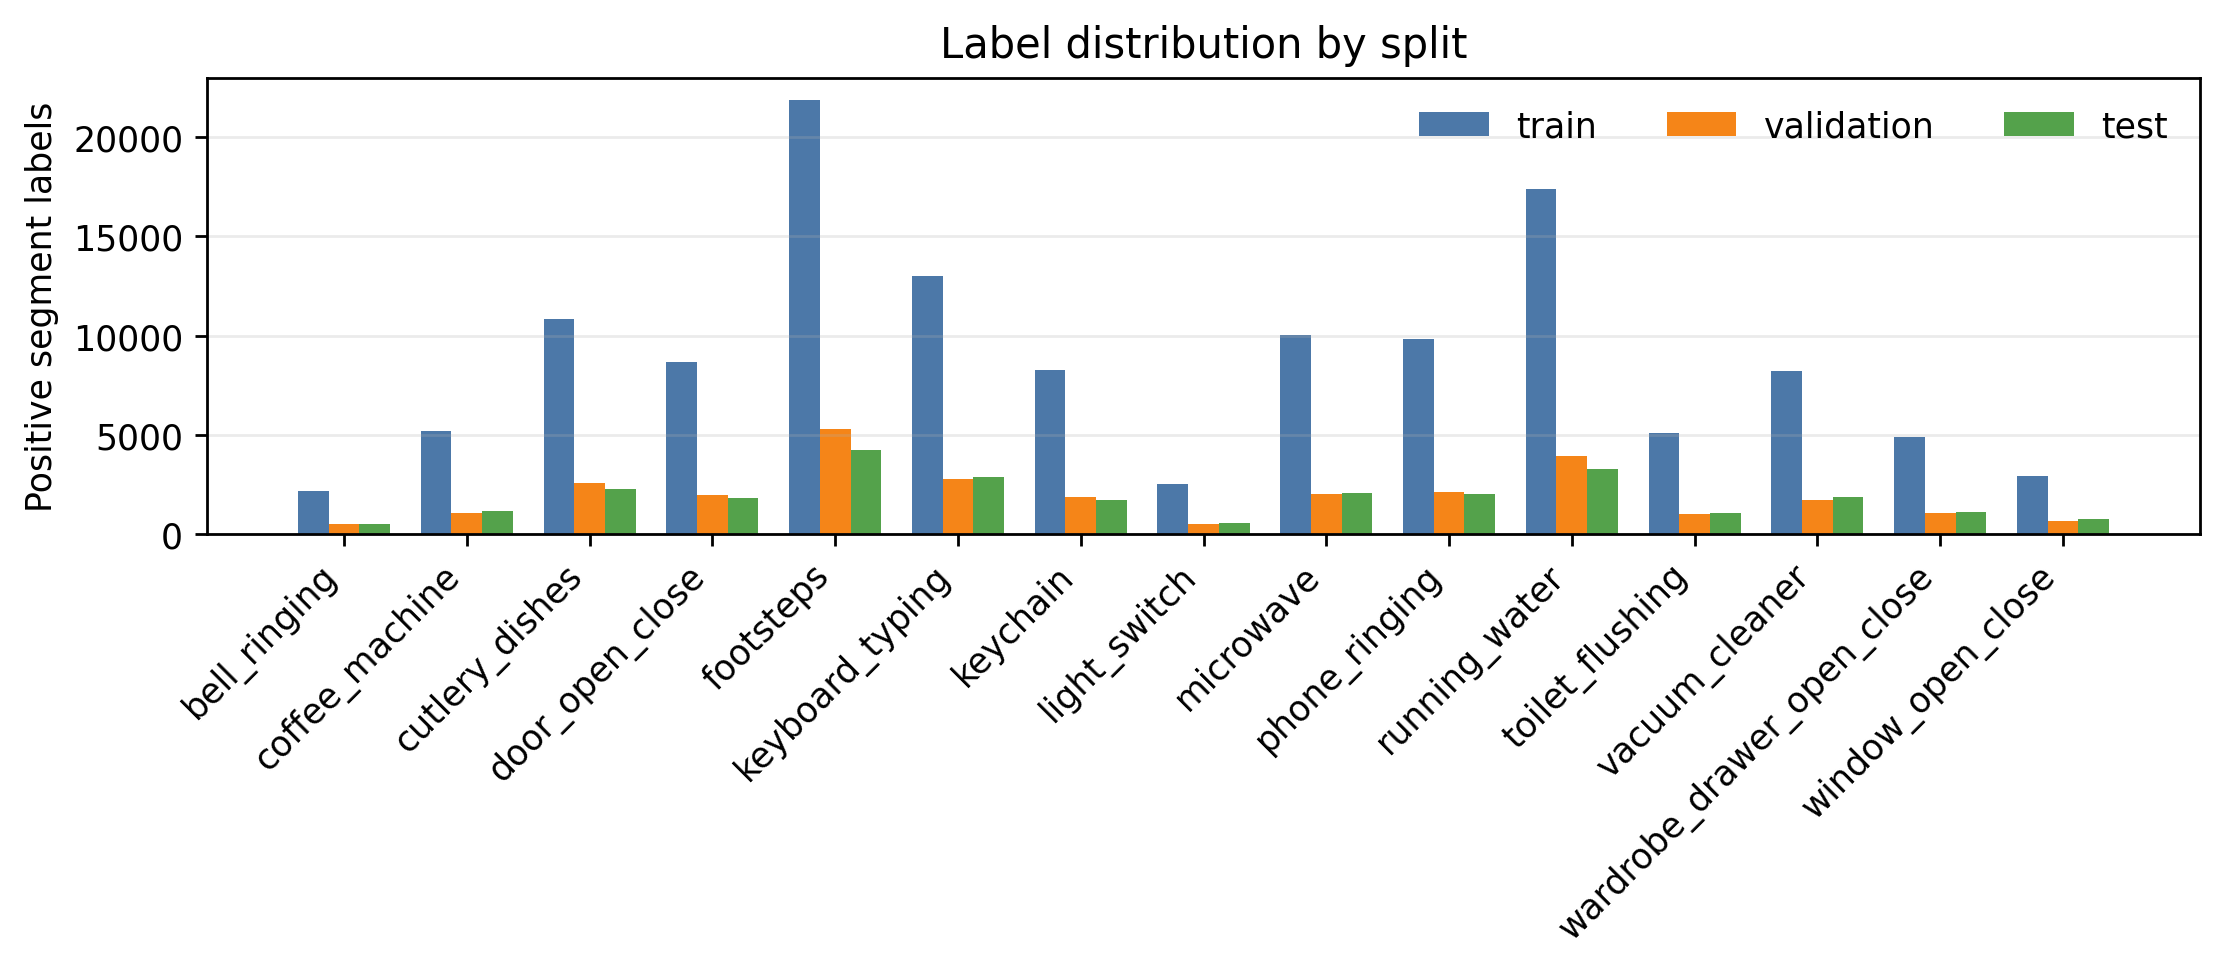
\includegraphics[width=\linewidth]{fig_label_distribution.png}
\caption{Positive segment labels per class and split.}
\end{figure}

\subsection{Train/Validation/Test Split}
We split data at recording level and also grouped by \texttt{collector\_id}.
This was feasible because every class remained present in all splits after the deterministic group search.
No recording or collector appears in more than one split.

\begin{table}[H]
\centering
\caption{Split summary.}
\begin{tabular}{lrrrr}
\toprule
Split & Recordings & Collectors & Segments & Label density\\
\midrule
train & 2564 & 286 & 117477 & 0.074 \\
validation & 549 & 61 & 25444 & 0.076 \\
test & 543 & 61 & 25318 & 0.072 \\
\bottomrule
\end{tabular}
\end{table}

\begin{figure}[H]
\centering
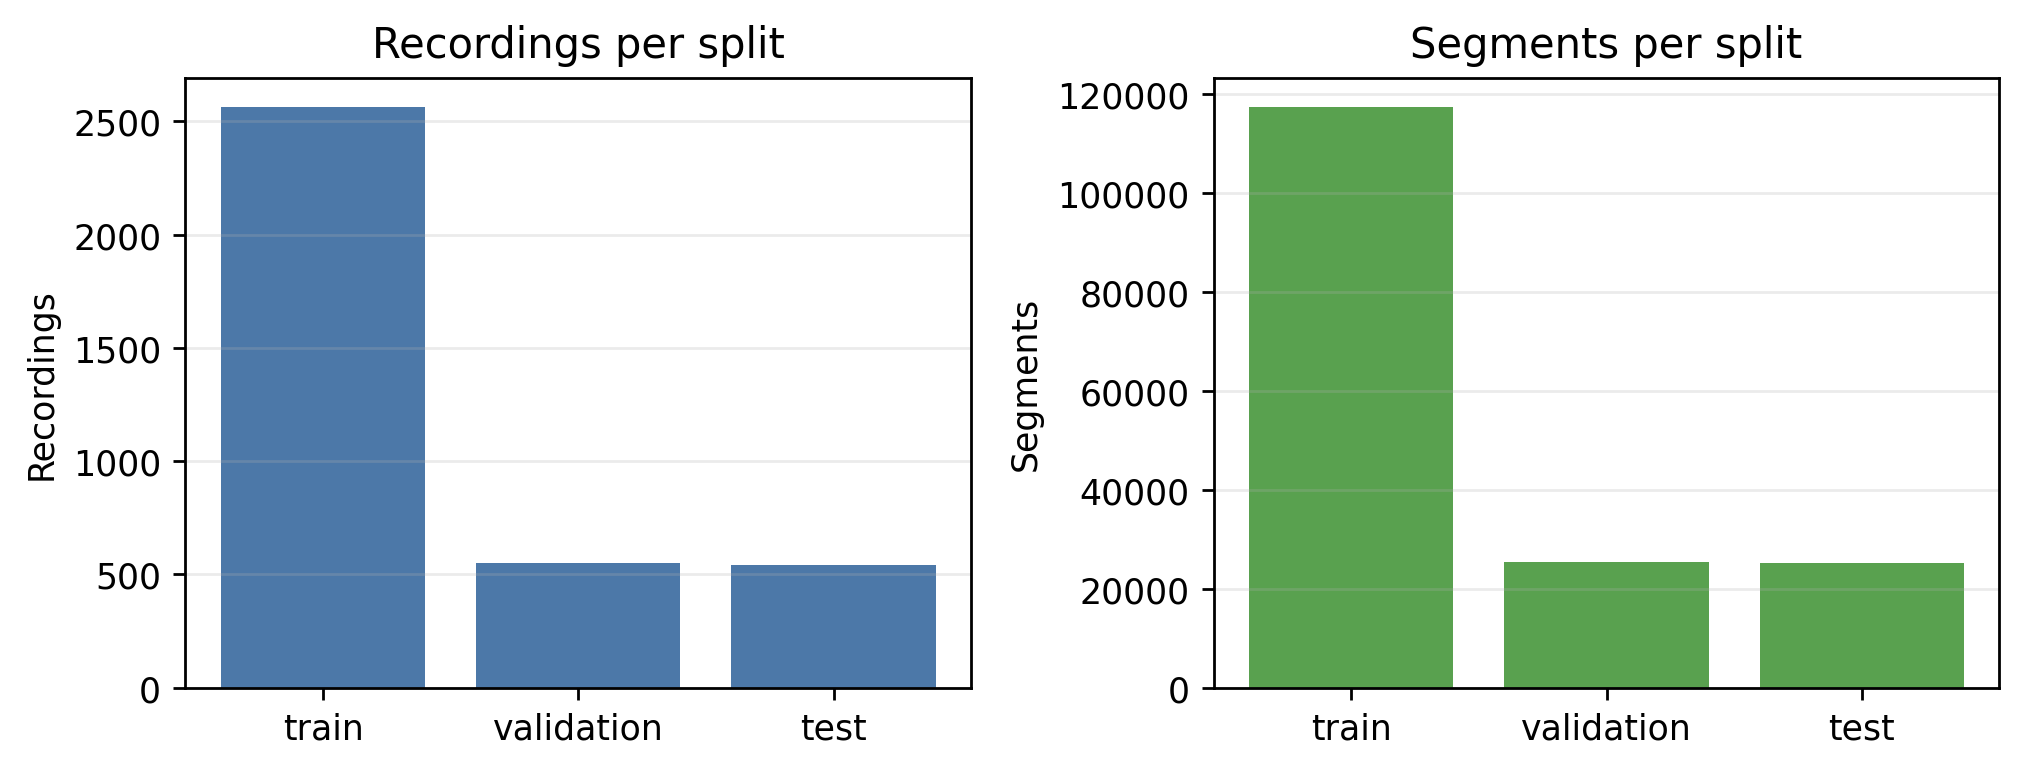
\includegraphics[width=\linewidth]{fig_split_distribution.png}
\caption{Number of recordings and segments in each split.}
\end{figure}

\subsection{Preprocessing}
We constructed segment-level matrices $X$ and $Y$.
The feature matrix concatenates 14 segment-level mean feature arrays, giving 240 features per segment.
Missing values were replaced with training-set medians.
Then all features were standardized with mean and variance estimated only on the training split.
The validation and test splits used the same fitted imputer and scaler.

\section{Evaluation}
\subsection{Metric Choice}
The main metric is Macro F1.
It gives equal weight to rare and frequent classes, which is important because the labels are imbalanced.
We also report Micro F1, which summarizes global segment-label decisions.
The theoretical best score is 1.0, but practical performance is limited by noisy labels, overlapping sound events, ambiguous sources, and uncertain temporal boundaries.

\subsection{Baseline}
We used an all-negative baseline and an empirical class-frequency baseline using only training prevalence.
On the test split, the all-negative baseline had Macro F1 0.000 and Micro F1 0.000.
The empirical baseline reached Macro F1 0.071 and Micro F1 0.096.

\section{Experiments}
\subsection{Classifiers and Hyperparameter Tuning}
We trained two model families: a one-vs-rest linear ridge classifier and a random forest.
Hyperparameters and the global decision threshold were selected on the validation set only.
The best validation configuration was \texttt{alpha=2.0} with threshold 0.50.

\begin{figure}[H]
\centering
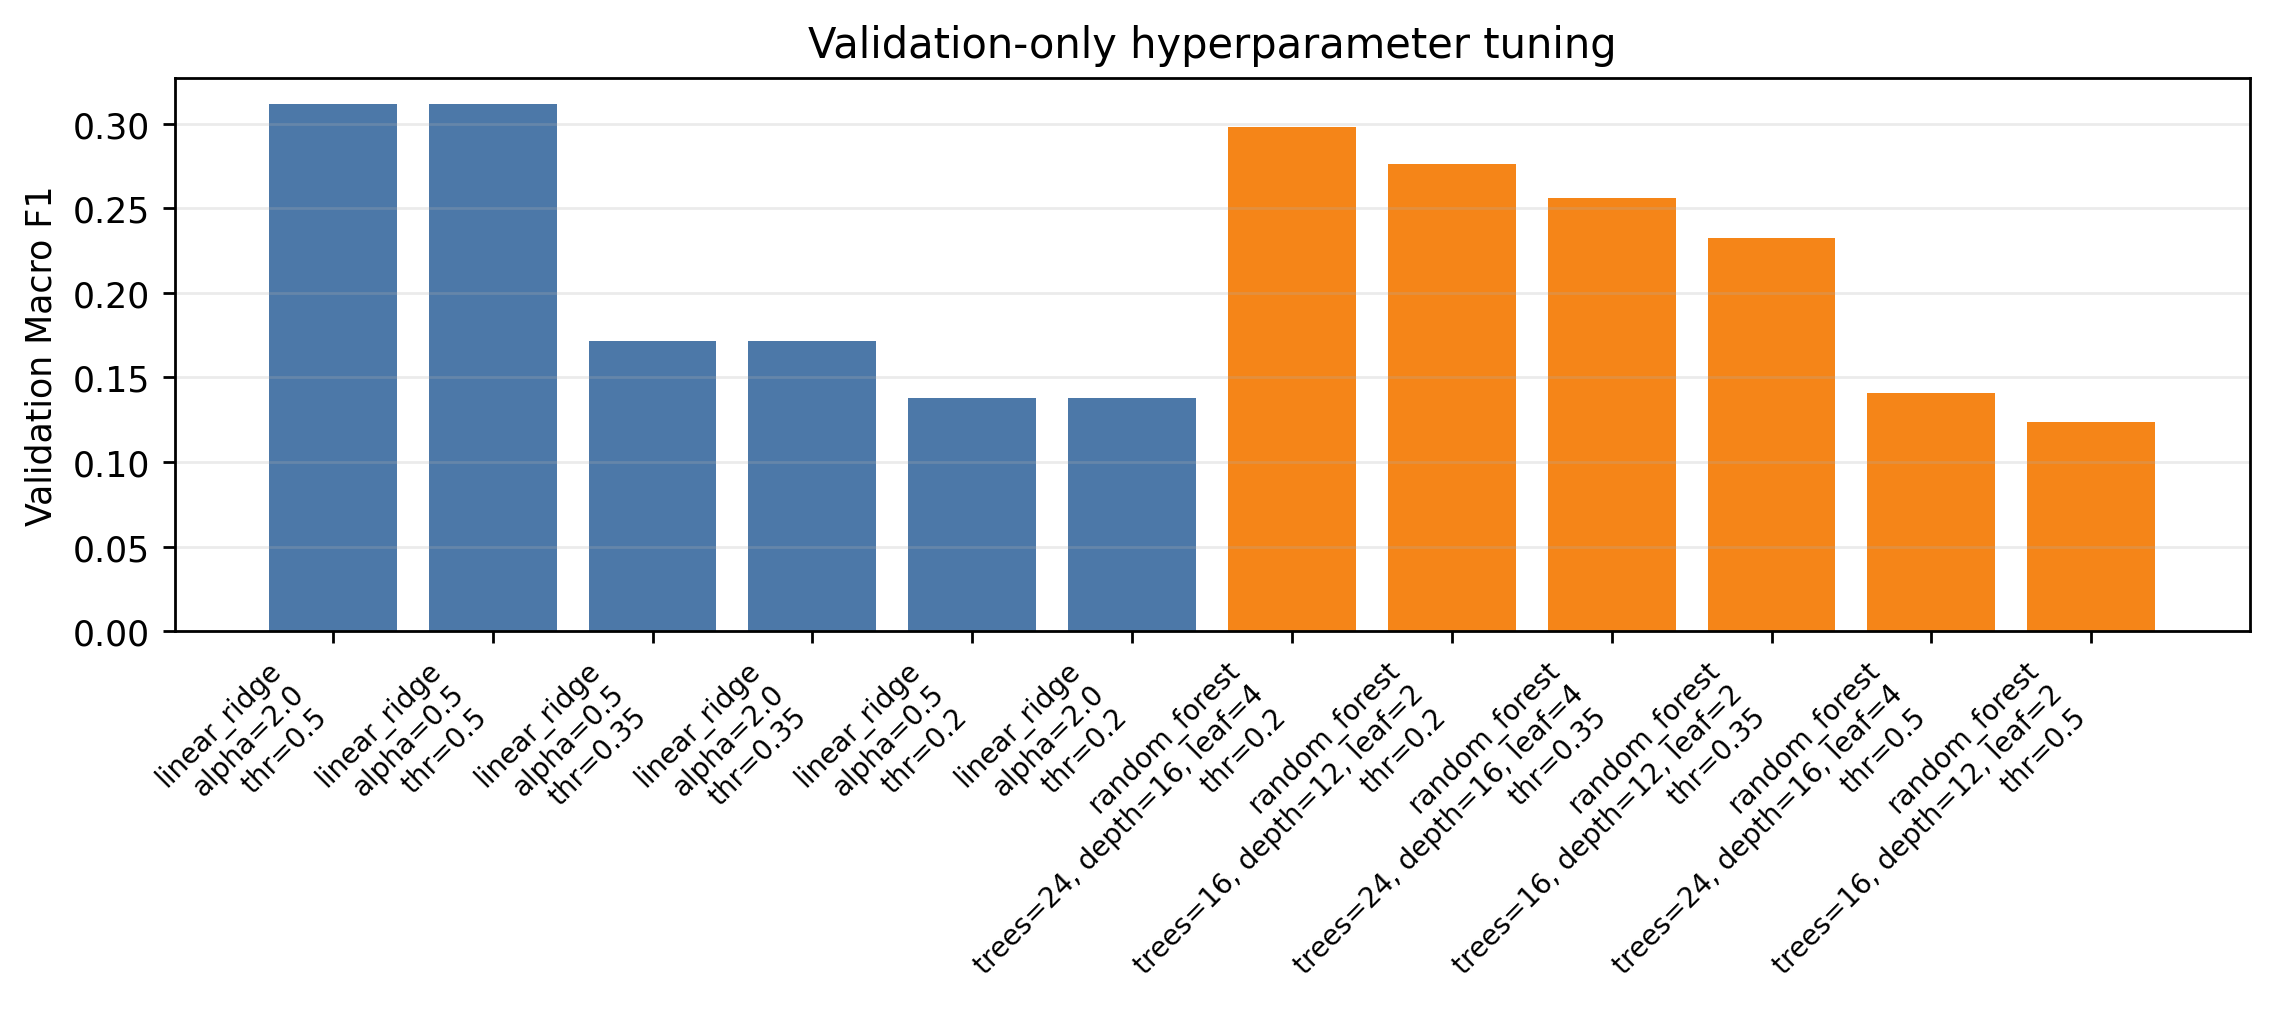
\includegraphics[width=\linewidth]{fig_hyperparameter_tuning.png}
\caption{Validation Macro F1 for tuned configurations.}
\end{figure}

\subsection{Final Results}
The selected final model was \texttt{linear\_ridge}.
It reached validation Macro F1 0.312 and test Macro F1 0.309.
Its validation Micro F1 was 0.308, and its test Micro F1 was 0.296.

\begin{table}[H]
\centering
\caption{Validation and test metrics.}
\begin{tabular}{lrrrr}
\toprule
Model & Val Macro F1 & Val Micro F1 & Test Macro F1 & Test Micro F1\\
\midrule
all\_negative & 0.000 & 0.000 & 0.000 & 0.000 \\
empirical\_frequency & 0.075 & 0.105 & 0.071 & 0.096 \\
linear\_ridge & 0.312 & 0.308 & 0.309 & 0.296 \\
random\_forest & 0.298 & 0.323 & 0.295 & 0.308 \\
\bottomrule
\end{tabular}
\end{table}

\begin{figure}[H]
\centering
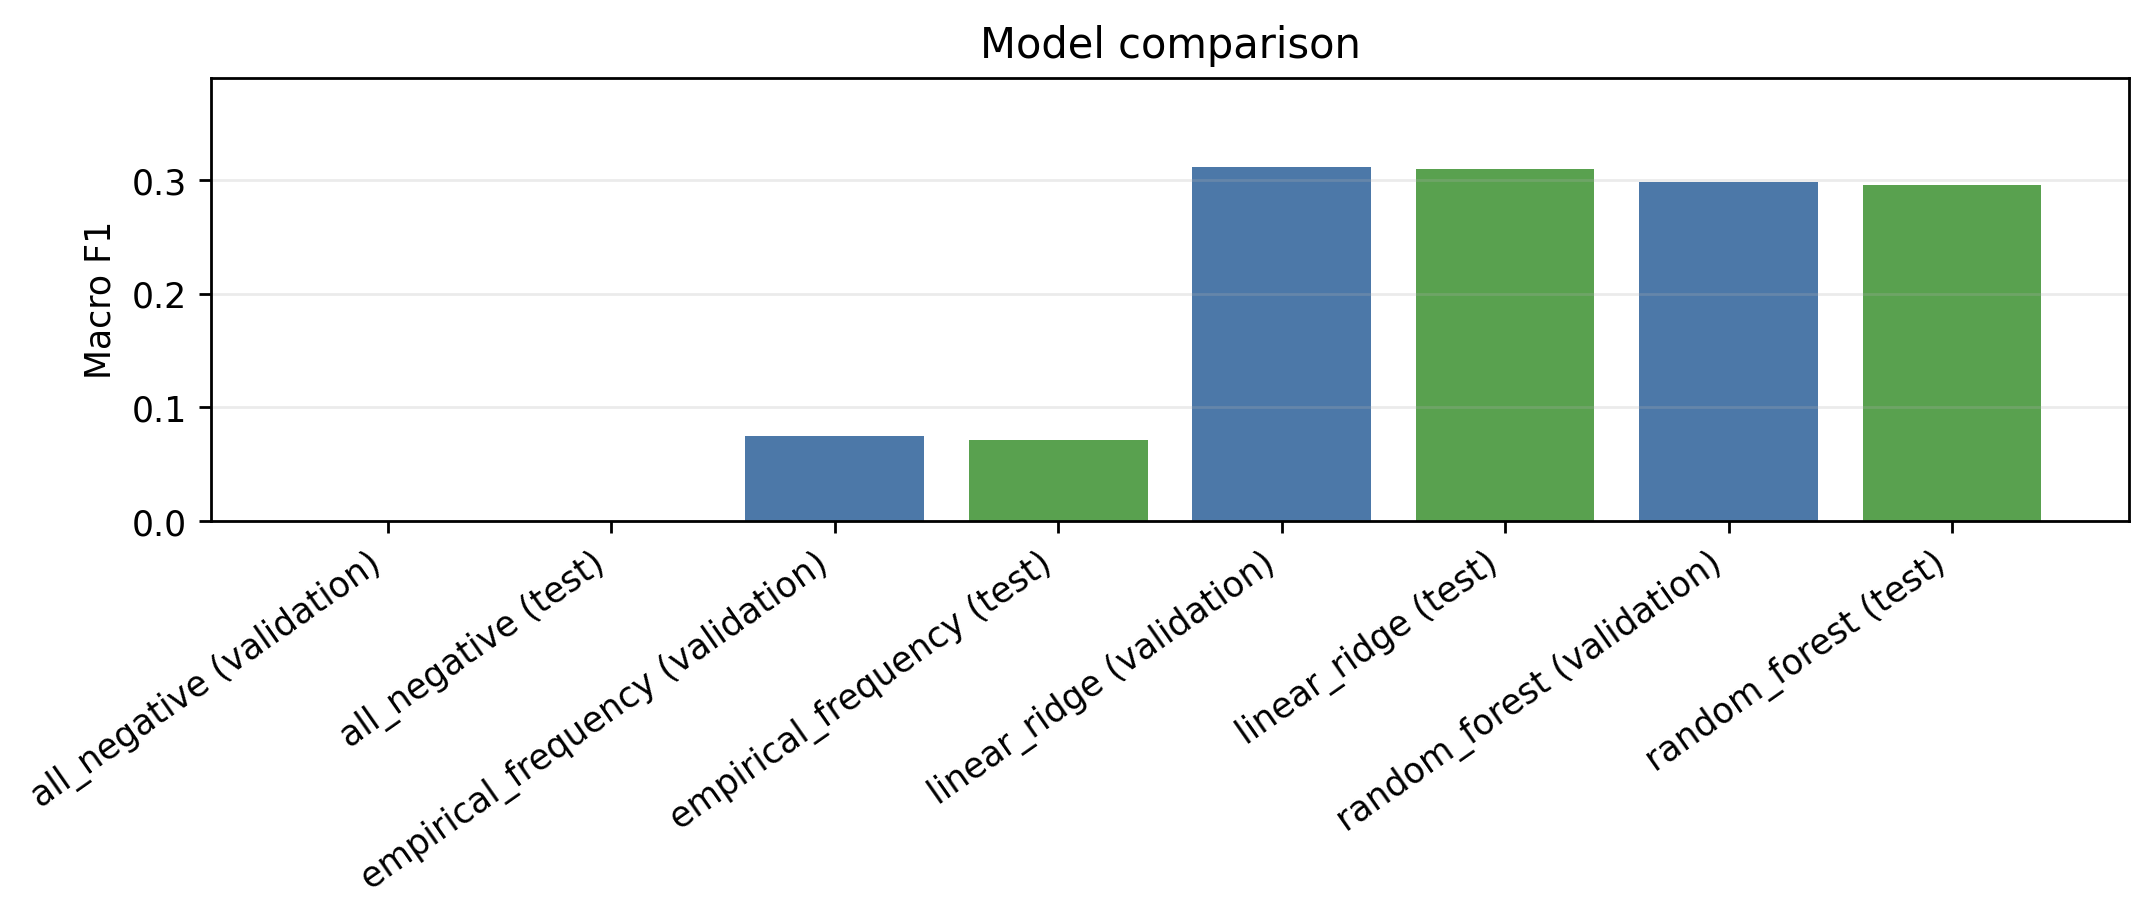
\includegraphics[width=\linewidth]{fig_model_comparison.png}
\caption{Macro F1 comparison across baselines and classifiers.}
\end{figure}

\begin{figure}[H]
\centering
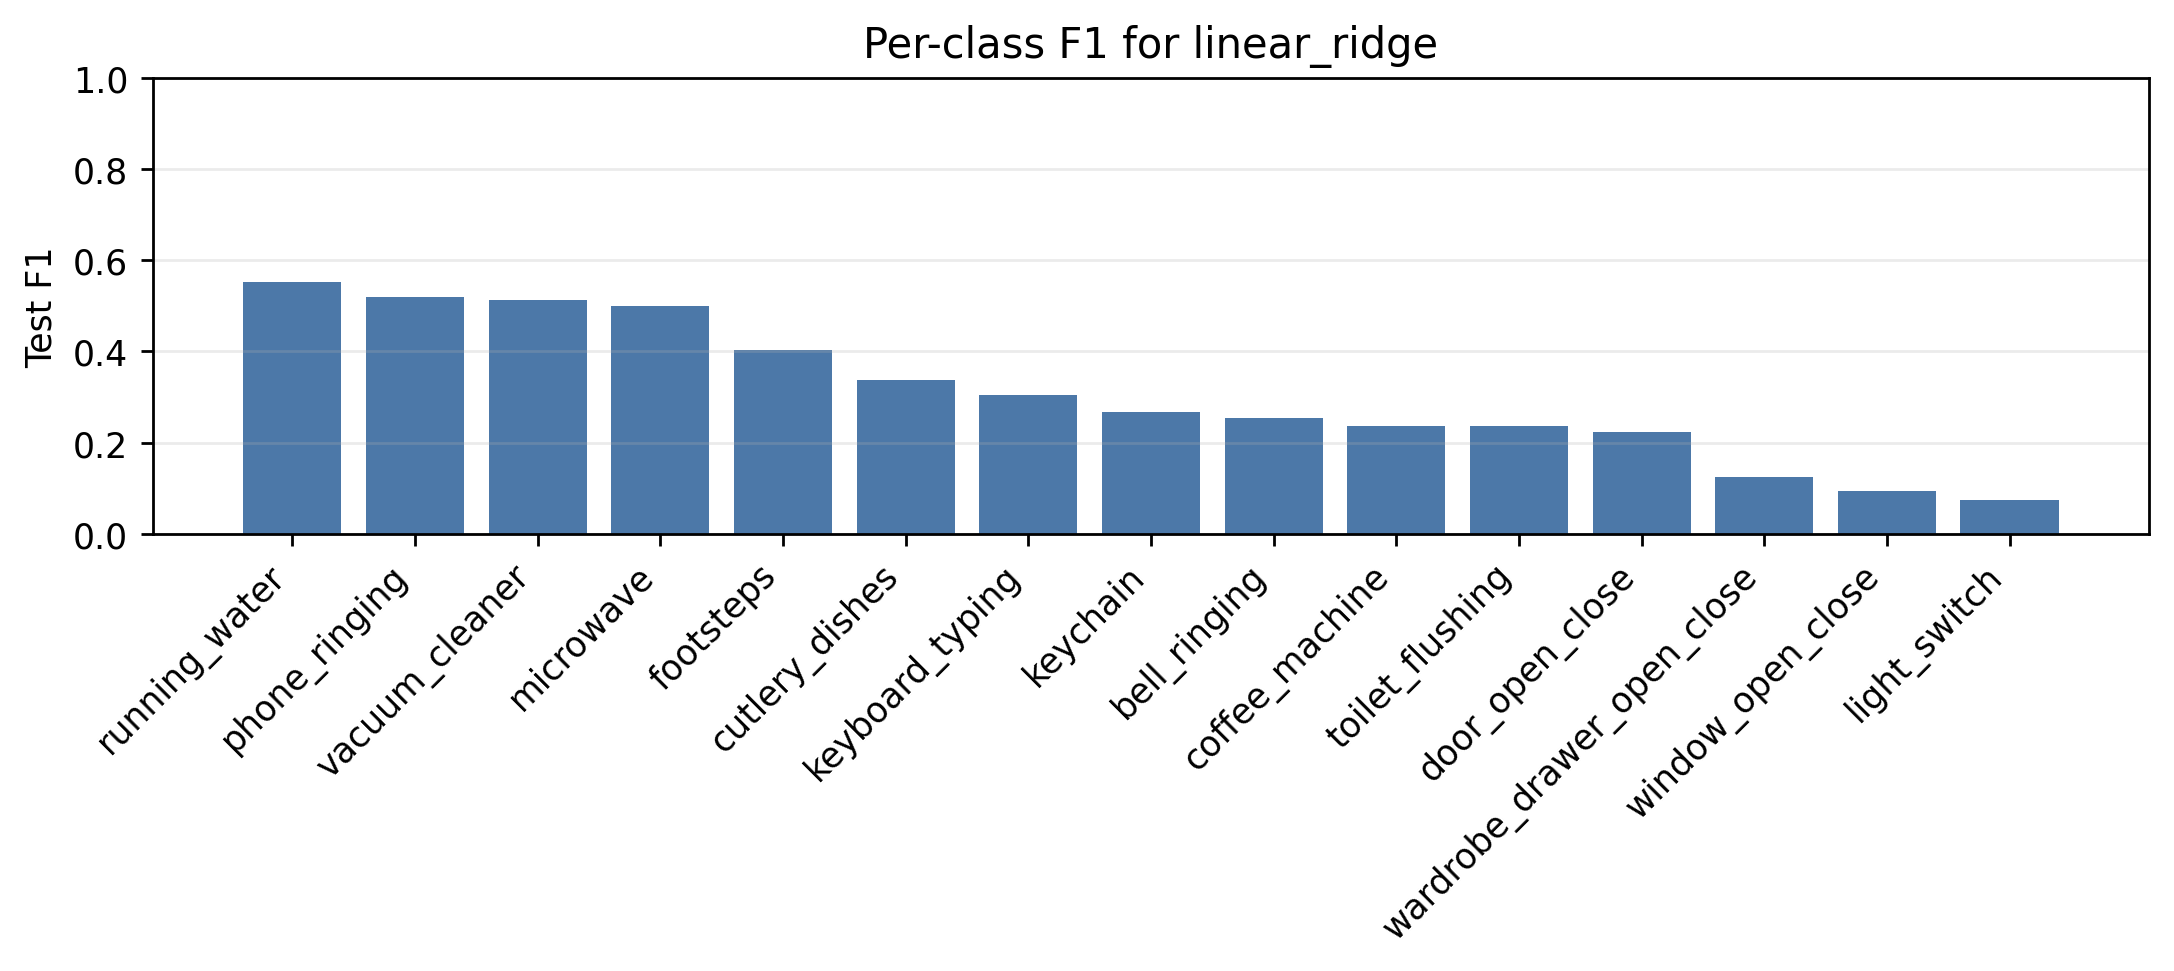
\includegraphics[width=\linewidth]{fig_per_class_f1.png}
\caption{Per-class test F1 for the selected model.}
\end{figure}

The strongest classes on test were \texttt{running\_water}, \texttt{phone\_ringing}, \texttt{vacuum\_cleaner}.
The most difficult classes were \texttt{light\_switch}, \texttt{window\_open\_close}, \texttt{wardrobe\_drawer\_open\_close}.

\section{Case Study and Reflection}
\subsection{Case Study 1}
The first case is \texttt{004028.wav} from the test split.
It is a relatively successful example with file-level Micro F1 0.691.
The true active classes were \texttt{cutlery\_dishes}, \texttt{microwave}, \texttt{running\_water}, and the model predicted \texttt{coffee\_machine}, \texttt{cutlery\_dishes}, \texttt{microwave}, \texttt{phone\_ringing}, \texttt{running\_water}, \texttt{toilet\_flushing}, \texttt{vacuum\_cleaner}, \texttt{wardrobe\_drawer\_open\_close}, \texttt{window\_open\_close}.

\begin{figure}[H]
\centering
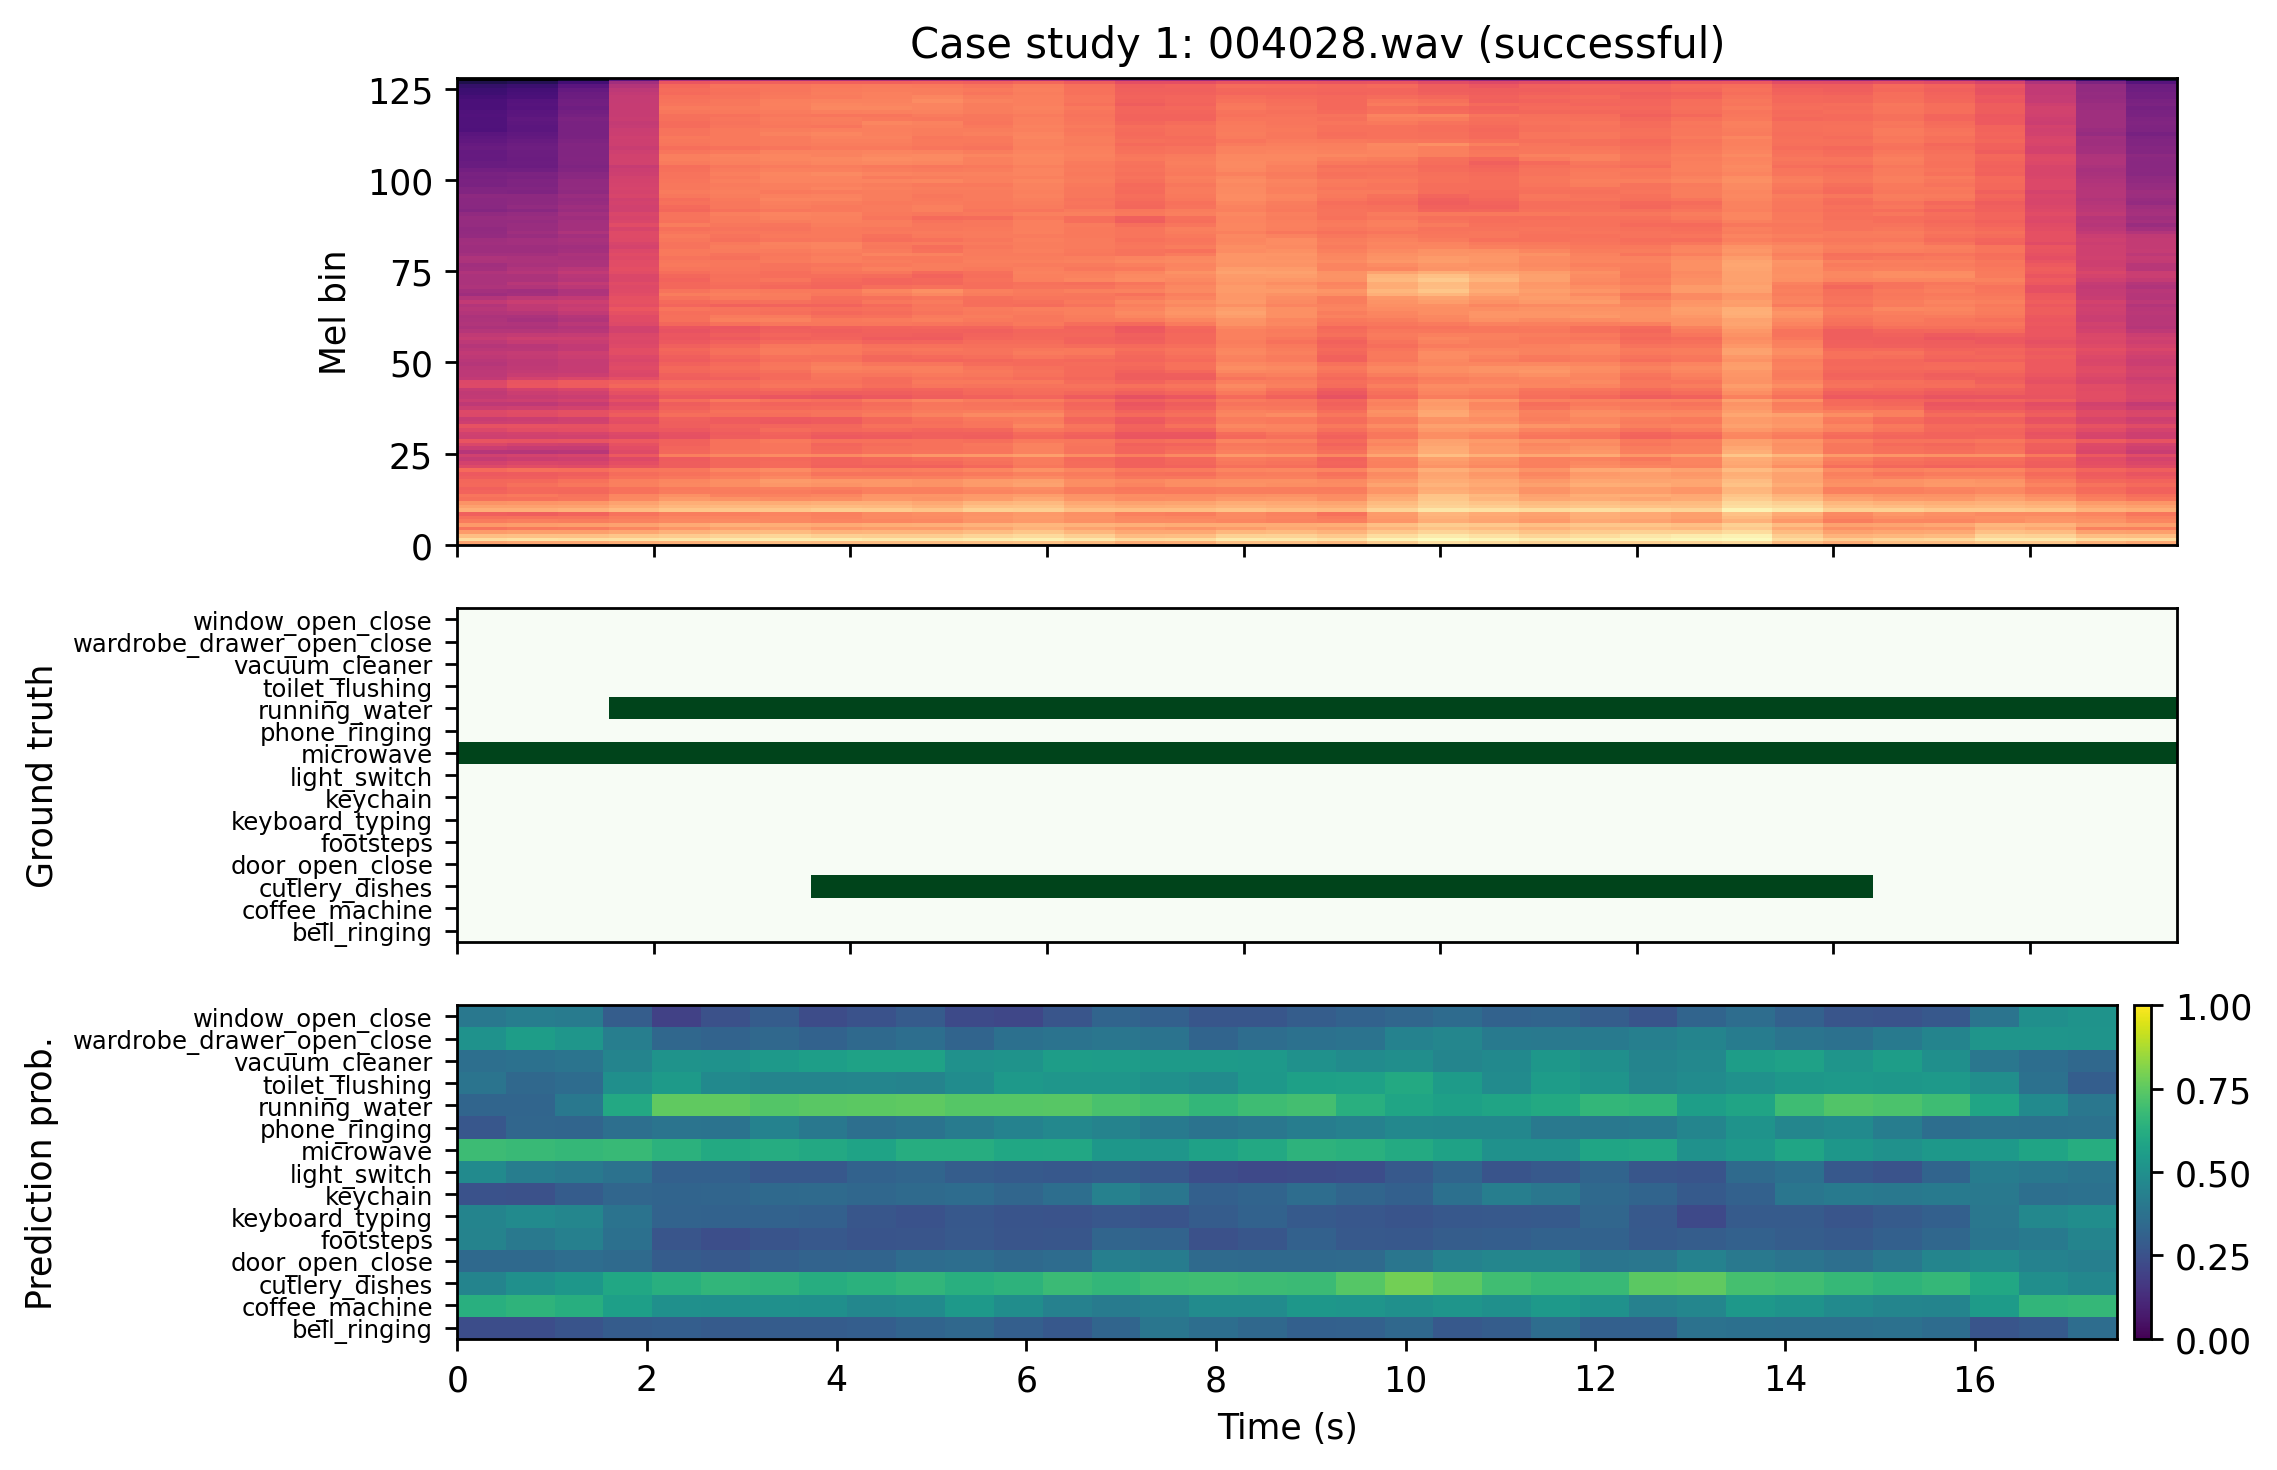
\includegraphics[width=\linewidth]{fig_case_study_1.png}
\caption{Successful case study: mel features, ground truth labels, and predicted probabilities.}
\end{figure}

\subsection{Case Study 2}
The second case is \texttt{005084.wav} from the test split.
It is a failure or ambiguous example with file-level Micro F1 0.000.
The true classes were \texttt{window\_open\_close}, while predicted classes were \texttt{coffee\_machine}, \texttt{door\_open\_close}, \texttt{footsteps}, \texttt{keyboard\_typing}, \texttt{microwave}, \texttt{wardrobe\_drawer\_open\_close}, \texttt{window\_open\_close}.
Missed classes were none; extra predicted classes were \texttt{coffee\_machine}, \texttt{door\_open\_close}, \texttt{footsteps}, \texttt{keyboard\_typing}, \texttt{microwave}, \texttt{wardrobe\_drawer\_open\_close}.

\begin{figure}[H]
\centering
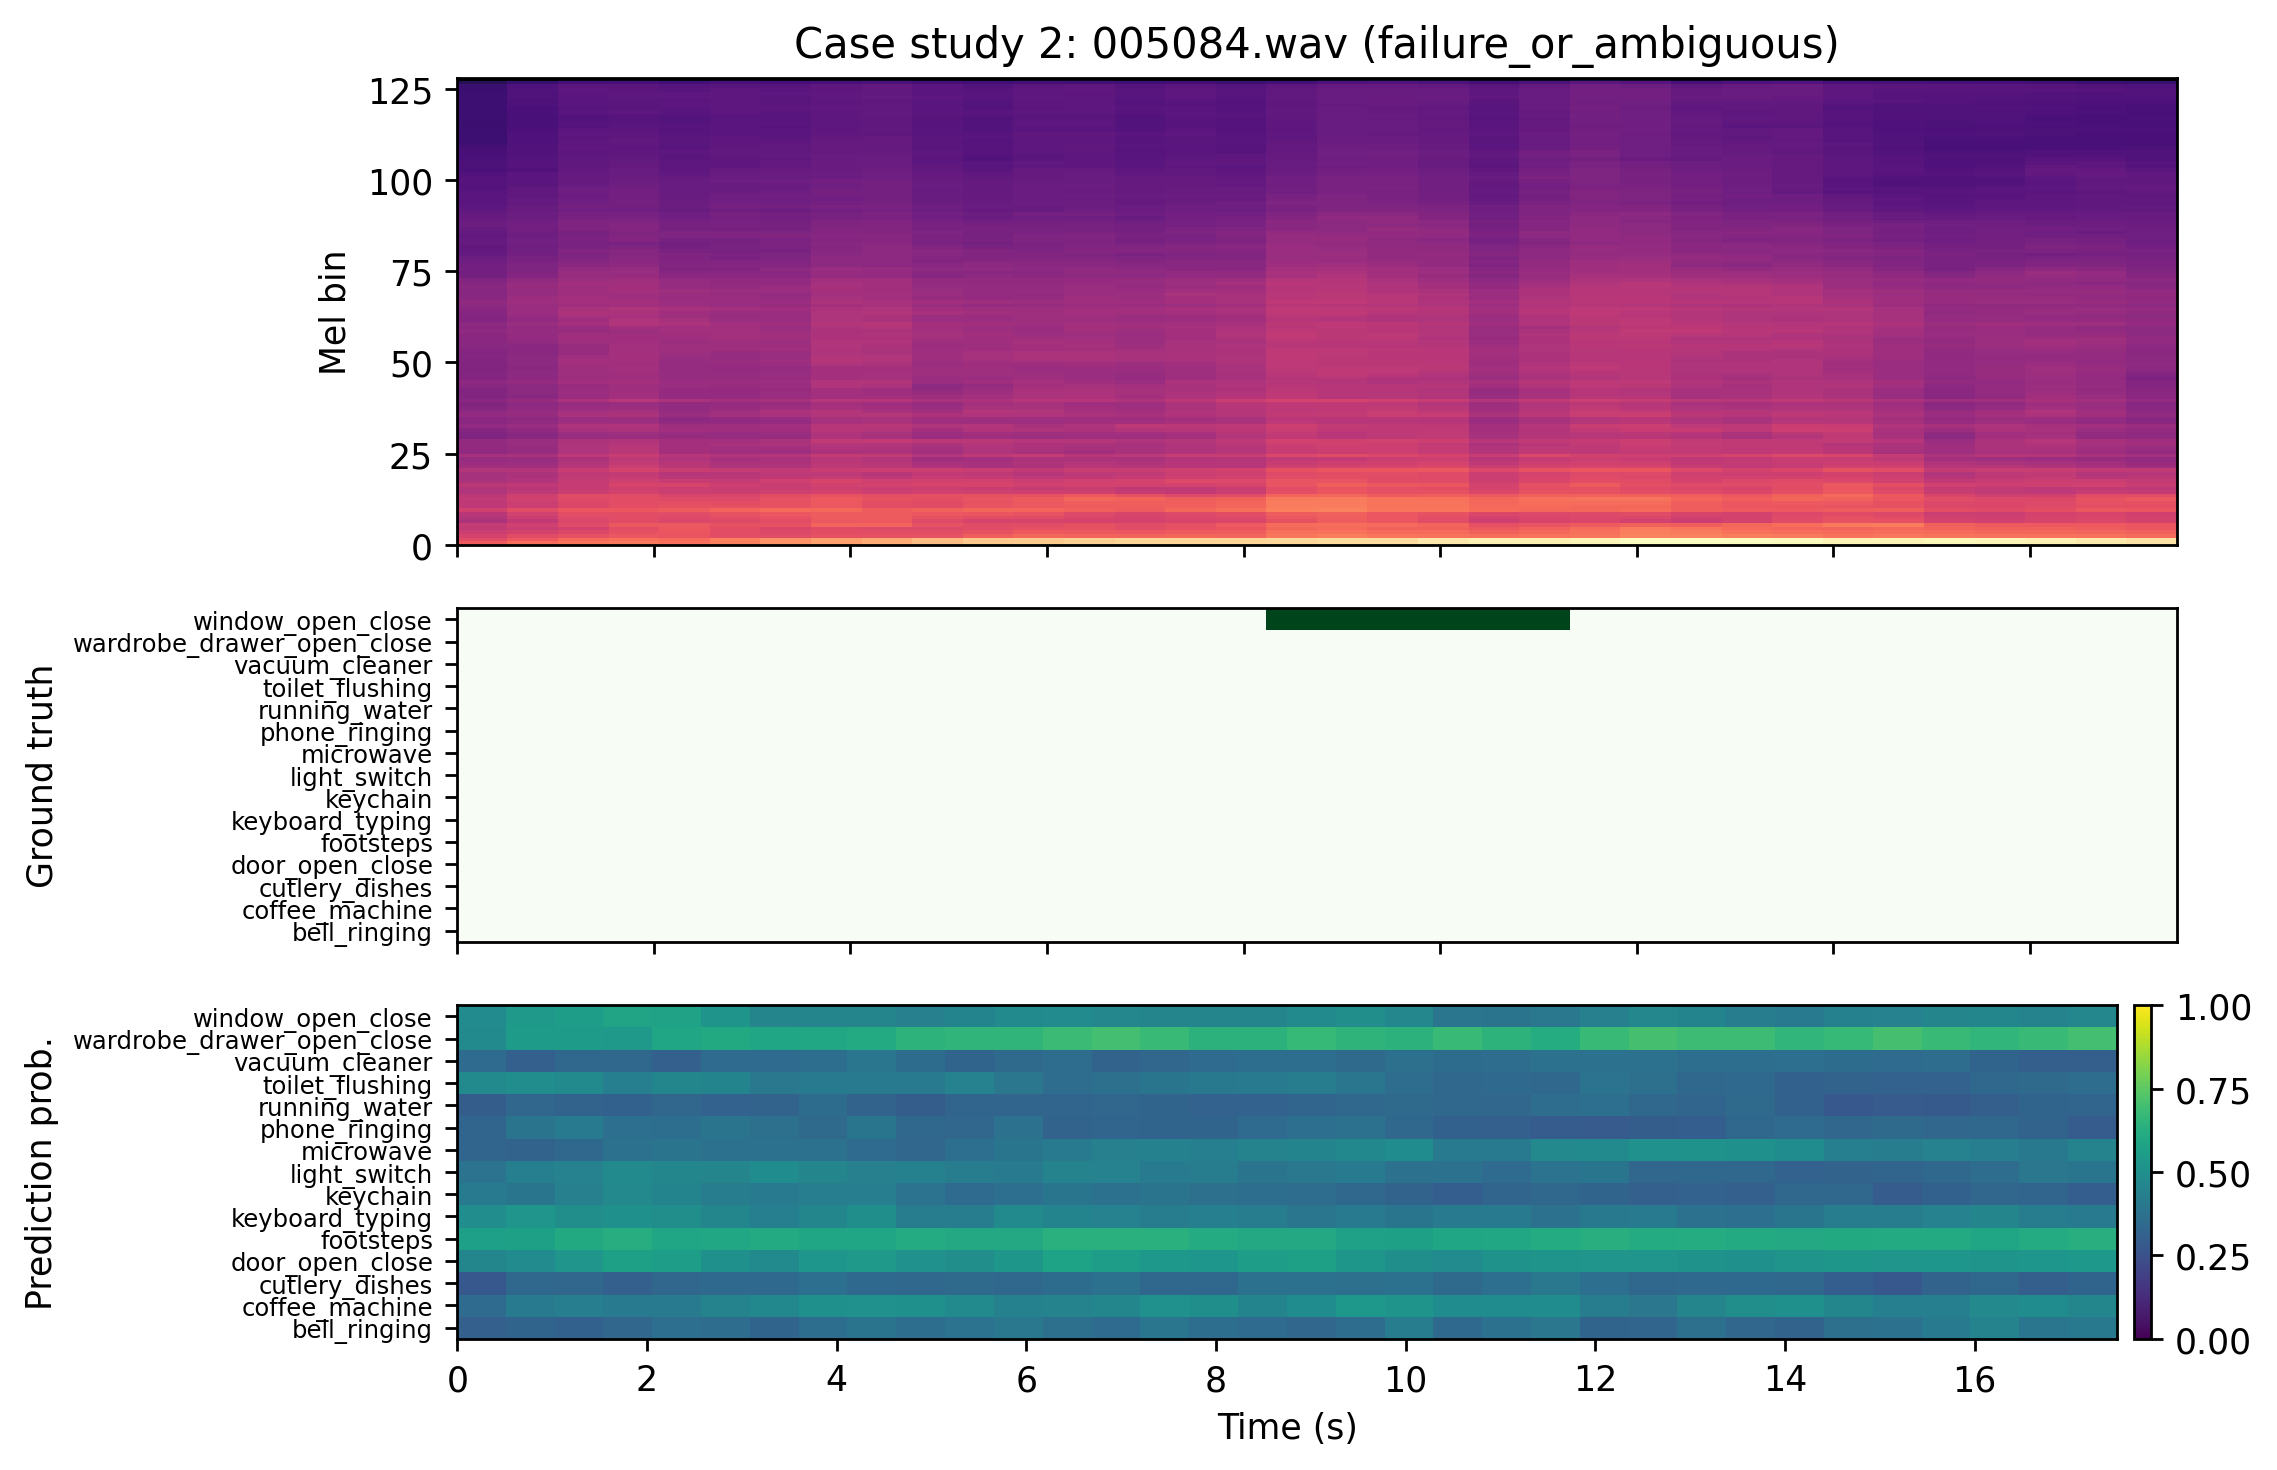
\includegraphics[width=\linewidth]{fig_case_study_2.png}
\caption{Failure or ambiguous case study with the same visualization format.}
\end{figure}

\subsection{Reflection}
The results show that the pipeline learns useful patterns, but the gap between classes is large.
Short transient classes and classes with similar acoustic texture are harder.
The model also uses segment features without long temporal context, so it can miss boundaries or confuse overlapping sounds.
A future improvement would tune class-specific thresholds and add temporal smoothing, still using validation data only.

\section{Disclosure of LLM and AI Tool Use}
We used ChatGPT/Codex to support planning, coding, debugging, and wording of the report.
All numerical results, plots, and interpretations were produced from the provided dataset and checked against the generated notebook outputs.

\end{document}
